% =====================================================================
%  §5. Корреляция как свойство плана эксперимента
%
%  ЖАНР (STYLE.md): учебная литература. Ни путей, ни имён программ, ни
%  номеров гипотез. Прослеживаемость — ключи \srckey{5.x} и приложение.
%
%  Содержательная основа: research/two_wgp/NOTE_malus_linearization.md §6;
%  BRIEF_FOR_D_teaching_ladder.md §6.
% =====================================================================
\section{Корреляция как свойство плана эксперимента}
\label{sec:correlation}
\markboth{§\thesection. Корреляция}{}

Формула ковариации~\eqref{eq:normal-eq} из §4 содержит $(X^{\mathsf T}WX)^{-1}$~--- матрицу,
целиком построенную из \emph{углов измерения} и весов, но не из самих измеренных значений. Это
не техническая деталь, а содержательный факт, который стоит вынести в отдельный параграф:
\textbf{насколько хорошо будут разделены параметры подгонки, известно ДО того, как получена хотя
бы одна точка данных}~--- достаточно знать, на каких углах прибор будет измерять. Здесь этот факт
проверяется на числах, вычислимых в закрытой форме, а в §9 тот же самый механизм вернётся в
гораздо менее наглядном виде~--- как вырождение параметров нелинейной модели.

\begin{tcolorbox}[enhanced,colback=cPanel,colframe=cGrid,boxrule=0.8pt,arc=2pt,
                  title={\bfseries\color{cAccent} Пререквизиты},coltitle=cAccent,
                  attach boxed title to top left={xshift=6pt,yshift=-2pt},
                  boxed title style={colback=cPanel,boxrule=0pt,arc=0pt},top=10pt]
\textbf{Нужно знать:} §4 целиком (матрица плана, нормальные уравнения, ковариация); что такое
собственные числа симметричной матрицы (на уровне интуиции: направления, в которых квадратичная
форма растёт быстрее или медленнее всего).\\[0.3em]
\textbf{Знать НЕ нужно:} численные методы решения плохо обусловленных систем~--- этот параграф про
то, как \emph{обнаружить} плохую обусловленность и что она означает, а не про то, как с ней
бороться вычислительно.
\end{tcolorbox}

% ---------------------------------------------------------------------
\subsection{Число обусловленности: одна цифра про качество плана}
\label{subsec:condition-number}

\begin{intuition}
Представьте матрицу $X^{\mathsf T}X$ как эллипсоид: чем он более вытянут, тем труднее по данным
различить движение вдоль его длинной оси от движения вдоль короткой~--- шум в любом направлении
неотличим от смеси обоих. \term{Число обусловленности} $\cond(X^{\mathsf T}X)$~--- отношение
наибольшего собственного числа к наименьшему~--- одним числом измеряет, насколько вытянут этот
эллипсоид. Число, близкое к единице,~--- эллипсоид почти круглый, направления равноправны; число,
на порядки больше единицы,~--- эллипсоид сильно вытянут, и в его <<узком>> направлении оценка
параметра ненадёжна, сколько бы ни было данных.
\end{intuition}

\begin{strict}
Для матрицы плана со столбцами $\{1,\cos2\theta,\sin2\theta,\cos4\theta,\sin4\theta\}$
обусловленность $X^{\mathsf T}X$ зависит только от того, \emph{на каких углах} стоят строки~---
то есть исключительно от плана измерения. Если столбцы (как функции на множестве измеренных
углов) взаимно ортогональны, $X^{\mathsf T}X$ диагональна и $\cond=1$; чем ближе какая-либо пара
столбцов к линейной зависимости (коллинеарности) на данном наборе углов, тем больше
$\cond(X^{\mathsf T}X)$, и тем хуже определены соответствующие коэффициенты.
\end{strict}

% ---------------------------------------------------------------------
\subsection{Две конфигурации одного и того же прибора}
\label{subsec:two-configs}

В проекте, на данных которого строится курс, угловая развёртка снималась либо на полном
симметричном диапазоне (примерно от $-90^\circ$ до $+90^\circ$), либо, в одном из режимов работы
установки, только на половине~--- от $0^\circ$ до $90^\circ$. Разница выглядит невинно: тот же шаг
по углу, просто вдвое меньше точек. Чистая геометрия матрицы плана говорит другое.

\begin{example}[: цена усечения диапазона, посчитанная без единого измерения]\srckey{5.1}
\begin{center}
\footnotesize
\setlength{\tabcolsep}{7pt}
\begin{tabular}{@{}lrrr@{}}
\toprule
\textbf{План} & \textbf{Углов} & $\cond(X^{\mathsf T}X)$ & $\sigma(\theta_0)$ при шуме $1\,\%$\\
\midrule
$-90^\circ\ldots+90^\circ$        & 19 & $\mathbf{2{,}14}$   & $\mathbf{0{,}096^\circ}$ \\
$0^\circ\ldots90^\circ$ & 10 & $\mathbf{236{,}3}$  & $\mathbf{0{,}944^\circ}$ \\
\bottomrule
\end{tabular}
\end{center}
Обусловленность хуже в сто с лишним раз, а точность офсета~--- почти в десять. Оба числа получены
из одной лишь геометрии множества углов~--- \emph{до} какого-либо измерения.
\end{example}

\begin{intuition}[: откуда берётся разница]
На полном симметричном диапазоне вторая и четвёртая гармоники угла почти ортогональны как функции
на множестве измеренных точек~--- максимальное перекрытие между ними всего около
$5\,\%$\srckey{5.1}. На диапазоне, обрезанном с одной стороны, симметрия множества углов
нарушена, и то же самое перекрытие вырастает до $37\,\%$\srckey{5.1}~--- гармоники перестают быть
почти независимыми измерениями, и матрица плана вытягивается в эллипсоид.
\end{intuition}

% ---------------------------------------------------------------------
\begin{figure}[t]
  \centering
  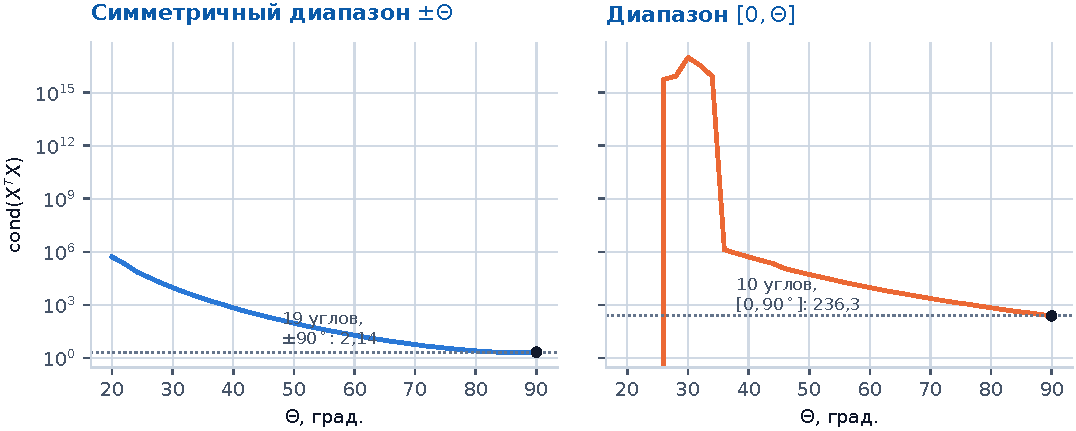
\includegraphics[width=\linewidth]{figures/fig05_cond_curve.pdf}
  \caption{Чистая геометрия матрицы плана (без каких-либо данных): $\cond(X^{\mathsf T}X)$ для
  пятигармонического базиса §4 как функция углового диапазона, при шаге между углами $10^\circ$.
  Слева: симметричный диапазон $\pm\Theta$. Справа: диапазон, зафиксированный с одной стороны в
  нуле, $[0,\Theta]$. Отмечены две конфигурации из таблицы примера~\ref{subsec:two-configs}.}
  \label{fig:cond-curve}
\end{figure}

% ---------------------------------------------------------------------
\subsection{Эллипс ковариации: та же геометрия, показанная напрямую}
\label{subsec:ellipse}

Число обусловленности~--- сводка одним числом; эллипс ковариации коэффициентов $(a_2,b_2)$
(§4) показывает ту же геометрию как картинку. При равном шуме на каждой точке эллипс с полными
осями, пропорциональными $\sqrt{\mathrm{собств.\,число\ }\operatorname{Cov}(a_2,b_2)}$, задаёт
область, где статистически неразличимы разные пары коэффициентов~--- а значит, и разные пары
(амплитуда второй гармоники, офсет).

\begin{figure}[t]
  \centering
  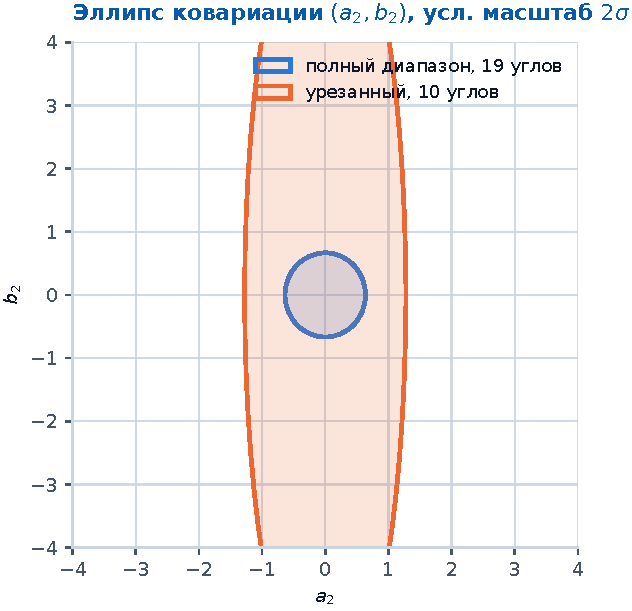
\includegraphics[width=0.82\linewidth]{figures/fig05_cov_ellipse.pdf}
  \caption{Эллипсы ковариации коэффициентов $(a_2,b_2)$ для двух планов таблицы
  примера~\ref{subsec:two-configs} (чистая геометрия $(X^{\mathsf T}X)^{-1}$ при единичном и
  одинаковом для всех точек шуме; масштаб эллипсов условный, важна их форма и вытянутость, а не
  абсолютный размер). Почти круглый эллипс полного диапазона против сильно вытянутого эллипса
  урезанного~--- то же число обусловленности, показанное геометрически.}
  \label{fig:cov-ellipse}
\end{figure}

% ---------------------------------------------------------------------
\subsection{Следствие: коллинеарность столбцов стоит вполне определённой цены}
\label{subsec:consequence}

Плохая обусловленность~--- не только про размер ошибки. У неё есть более коварное следствие:
если модель, применённая к плохо обусловленному плану, случайно \emph{забывает} один из
почти-коллинеарных столбцов (например, отбрасывает четвёртую гармонику, как это делает учебная
трёхпараметрическая форма §\ref{subsec:idea}), то оставшийся столбец вынужден скомпенсировать её
вклад~--- и оценка получает \term{систематическое смещение}, а не просто увеличенный разброс.

\begin{example}[: смещение офсета от одной лишь обрезки диапазона]\srckey{5.2}
На реальных развёртках сдвиг оценки офсета при переходе с полного диапазона на урезанный
составил:
\begin{center}
\footnotesize
\setlength{\tabcolsep}{7pt}
\begin{tabular}{@{}lr@{}}
\toprule
\textbf{Образец} & \textbf{Сдвиг $\theta_0$, полный $\to$ урезанный} \\
\midrule
плотная решётка, $D/P=0{,}71$        & $-0{,}687^\circ$ \\
повторная установка, $D/P=0{,}69$ (а) & $+0{,}351^\circ$ \\
повторная установка, $D/P=0{,}69$ (б) & $-2{,}103^\circ$ \\
разреженный образец, $D/P=0{,}46$    & $-0{,}920^\circ$ \\
\bottomrule
\end{tabular}
\end{center}
Величина сдвига~--- не шум измерения, а прямое следствие геометрии плана: она того же порядка,
что и обсуждаемые в проекте расхождения между конкурирующими оценками углового офсета,
полученными совсем другими методами. Иными словами, часть того, что могло бы показаться
содержательным физическим расхождением, оказывается артефактом одного лишь выбора углов
измерения.
\end{example}

\begin{warning}[: это не довод против урезанного диапазона как такового]
Урезанный диапазон~--- не ошибка сам по себе; в некоторых установках он вынужден геометрией
прибора. Проблема~--- не в его использовании, а в применении к нему модели, которая \emph{не
учитывает} все гармоники, необходимые для точного описания наблюдаемой (§\ref{subsec:idea}).
Если модель включает все пять коэффициентов, оценки остаются несмещёнными на любом диапазоне~---
меняется только их точность (столбец $\sigma(\theta_0)$ таблицы примера~\ref{subsec:two-configs}),
а не их центр.
\end{warning}

% ---------------------------------------------------------------------
\subsection{Мост к нелинейной задаче}
\label{subsec:bridge}

\begin{tcolorbox}[enhanced,colback=cS1!7,colframe=cS1,boxrule=0pt,leftrule=3pt,arc=1pt]
\textbf{Главная мысль параграфа, которая пригодится во всей оставшейся части курса.} Если два
столбца матрицы плана почти коллинеарны на множестве измеренных точек, соответствующие им
параметры \emph{почти неразличимы}: данные знают только их определённую комбинацию, а не каждый
параметр по отдельности. Это верно для линейной задачи, где всё считается в закрытой форме и
видно на эллипсе. В §§6--7 модель перестанет быть линейной по параметрам, замкнутой формулы для
ковариации больше не будет, и вместо матрицы плана~$X$ появится \term{якобиан} модели,
вычисленный в точке минимума. Но геометрический смысл~--- тот же самый: почти параллельные
столбцы якобиана означают почти неразличимые параметры. Именно этим механизмом в §9 объясняется
вырождение $\Deff\leftrightarrow\eta_0\leftrightarrow\varepsilon_{\rm cross}$~--- то же самое
явление, что в этом параграфе можно было увидеть глазом на эллипсе, просто в применении к
нелинейной модели, где эллипс уже не рисуется одной формулой.
\end{tcolorbox}

% ---------------------------------------------------------------------
\subsection{Типичные ошибки этого параграфа}

\begin{enumerate}[leftmargin=1.6em,itemsep=0.25em]
  \item Считать корреляцию параметров свойством \emph{данных} или метода подгонки. Она сидит в
        $(X^{\mathsf T}WX)^{-1}$, а $X$ строится только из углов измерения~--- корреляцию можно
        вычислить заранее, при планировании эксперимента.
  \item Путать увеличенную ошибку (разброс) со смещением (сдвигом центра оценки). Плохая
        обусловленность сама по себе даёт первое; смещение возникает только тогда, когда модель
        вдобавок отбрасывает один из почти-коллинеарных столбцов (§\ref{subsec:consequence}).
  \item Обрезать угловой диапазон и не пересмотреть при этом набор гармоник в модели. Урезанный
        диапазон не запрещён, но требует более осторожного отношения к тому, какие члены модели
        ещё различимы на нём.
  \item Считать, что вырождение параметров бывает только в нелинейных задачах. Это в первую
        очередь линейный эффект, который в линейной задаче виден напрямую~--- в нелинейной он
        просто прячется в якобиане (§\ref{subsec:bridge}).
\end{enumerate}

\clearpage
